% =====================================================================
%  Sensa — Wearable Air Quality Monitoring System with Embedded AI
%  Cal Poly EE Senior Project Poster (48" x 36", landscape)
%
%  Build with:  latexmk -pdf -xelatex poster.tex
%        or:    xelatex poster.tex   (twice for refs)
% =====================================================================
\documentclass[final,t]{beamer}

\usepackage[size=custom,width=121.92,height=91.44,scale=1.25]{beamerposter} % 48" x 36"
\usepackage[utf8]{inputenc}
\usepackage{lmodern}
\usepackage{microtype}
\usepackage{graphicx}
\usepackage{tikz}
\usetikzlibrary{positioning, arrows.meta, fit}
\usepackage{adjustbox}
\usepackage{array,booktabs,tabularx}
\usepackage{ragged2e}
\usepackage{enumitem}
\usepackage{xcolor}
\usepackage{wrapfig}

% ---------- Cal Poly palette -----------------------------------------
\definecolor{cpgreen}{HTML}{154734}   % Cal Poly Green (PMS 343)
\definecolor{cpgold}{HTML}{BD8B13}    % Cal Poly Gold
\definecolor{cpsage}{HTML}{3F7A5E}    % lighter green for accents
\definecolor{cpcharcoal}{HTML}{2B2B2B}
\definecolor{cprule}{HTML}{B8B8B8}    % subtle horizontal rules
\definecolor{cpsand}{HTML}{F5F2EA}    % off-white block background

% ---------- Beamer color/styling -------------------------------------
\setbeamercolor{background canvas}{bg=white}
\setbeamercolor{normal text}{fg=cpcharcoal}
\setbeamercolor{itemize item}{fg=cpgreen}
\setbeamercolor{itemize subitem}{fg=cpsage}

\setbeamertemplate{itemize item}{\textcolor{cpgreen}{\textbullet}}
\setbeamertemplate{itemize subitem}{\textcolor{cpsage}{\textendash}}
% Belt-and-suspenders: also override via enumitem in case beamer template is suppressed
\setlist[itemize,1]{label=\textcolor{cpgreen}{\textbullet}, leftmargin=1.2em, labelsep=0.5em}
\setlist[itemize,2]{label=\textcolor{cpsage}{\textendash}, leftmargin=1.2em, labelsep=0.5em}
\setbeamertemplate{navigation symbols}{}

% Section header used inside each "card" --------------------------------
\newcommand{\sectionhead}[1]{%
  {\color{cpgreen}\bfseries\fontsize{40}{46}\selectfont #1}\\[0.1em]
  {\color{cpgold}\rule{\linewidth}{2pt}}\vspace{0.4em}\par
}

% A clean "card" container --------------------------------------------
\newenvironment{card}[1]
  {\begin{beamercolorbox}[wd=\linewidth,sep=0.8em,rounded=true,shadow=false]{}%
   \begin{minipage}{\linewidth}\sectionhead{#1}\justifying}
  {\end{minipage}\end{beamercolorbox}\vspace{0.6em}}

% Image placeholder ----------------------------------------------------
% \placeholder{aspect ratio width:height}{caption}
\newcommand{\placeholder}[3][\linewidth]{%
  \begin{tikzpicture}
    \node[draw=cprule,line width=1pt,fill=cpsand,minimum width=#1,
          minimum height=#2,align=center,inner sep=0pt,rounded corners=6pt]
      {\color{cpsage}\bfseries\fontsize{22}{26}\selectfont [\,#3\,]};
  \end{tikzpicture}\par
}

\newcommand{\figcap}[1]{\par\vspace{0.2em}{\color{cpcharcoal}\large\itshape Figure: #1}\par}

% =====================================================================
%  Title bar (custom — replaces beamer's default headline)
% =====================================================================
\newlength{\headerheight}\setlength{\headerheight}{11.5cm}
\newlength{\accentheight}\setlength{\accentheight}{0.5cm}

\setbeamertemplate{headline}{%
  \leavevmode
  \begin{tikzpicture}
    % Main green bar
    \fill[cpgreen] (0,0) rectangle (\paperwidth,\headerheight);
    % Thin gold accent strip directly below
    \fill[cpgold] (0,-\accentheight) rectangle (\paperwidth,0);
    % Title block (left)
    \node[anchor=west,inner sep=0pt,text=white] at (1.8cm,\headerheight/2){%
      \begin{minipage}{0.74\paperwidth}
        {\fontsize{82}{92}\selectfont\bfseries Wearable Air Quality Monitoring}\\[0.15em]
        {\fontsize{82}{92}\selectfont\bfseries System with Embedded AI}\\[0.5em]
        {\fontsize{34}{40}\selectfont Ryan Niemi \;\textbar\; Maddie Masiello \;\textbar\; Gulianna Corteguera}\\[0.15em]
        {\color{cpgold}\fontsize{30}{34}\selectfont\itshape Advisor: Mohammad Ghamari \quad\textbullet\quad California Polytechnic, Electrical Engineering}
      \end{minipage}};
    % Right-side institution block — Cal Poly logo + department name
    \node[anchor=east,inner sep=0pt,text=white] at (\paperwidth-1.8cm,\headerheight/2){%
      \begin{minipage}{0.20\paperwidth}\raggedleft
        
\includegraphics[width=0.18\paperwidth]{img/CP_logo_rev.png}\\[0.4em]
        {\color{cpgold}\fontsize{51}{57}\selectfont Electrical Engineering}
      \end{minipage}};
  \end{tikzpicture}\par\vspace{\accentheight}
}
\setbeamertemplate{footline}{%
  \leavevmode
  \begin{beamercolorbox}[wd=\paperwidth,ht=1.4cm,dp=0.4cm,leftskip=2cm,rightskip=2cm]{}
    \color{cpcharcoal}\small
    \textbf{Sensa} \textbullet\; California Polytechnic Electrical Engineering Senior Project 2025--2026
  \end{beamercolorbox}
}

% =====================================================================
\begin{document}
\begin{frame}[t]\vspace{0.5em}

\begin{columns}[t,totalwidth=\linewidth]

% =====================================================================
% LEFT COLUMN
% =====================================================================
\begin{column}{.315\linewidth}

\begin{card}{Motivation}
Most individuals live in areas where \textbf{accurate, real-time air-quality
information is unavailable}. Existing wearable monitors are limited by:
\begin{itemize}\setlength\itemsep{0.25em}
  \item Calibration drift and innacuracy in low-cost PM and VOC sensors
  \item Bulky form factors and \$300+ price points
\end{itemize}
\vspace{0.3em}
\textbf{Sensa} closes this gap with a compact, battery-powered, AI-driven
device that \emph{automatically self-calibrates} on-device, delivering
laboratory-grade awareness for everyday users.
\end{card}

\begin{card}{Project Objectives}
\begin{itemize}\setlength\itemsep{0.3em}
  \item Measure PM\textsubscript{2.5},
        PM\textsubscript{10}, VOC index, NO\textsubscript{x} index, temperature,
        and humidity in real time
  \item Run \textbf{embedded CNN calibration \& classification} entirely
        on-device
  \item Achieve \textbf{$\geq 12$~hour} battery life in a wearable
        (${<}\,3$~in\textsuperscript{2}) form factor
  \item Stay under a \textbf{\$100} bill-of-materials target
  \item Achieve accuracy similar to laboratory-grade reference equipment
\end{itemize}
\end{card}

\begin{card}{Hardware --- Custom Sensa PCB}
\centering
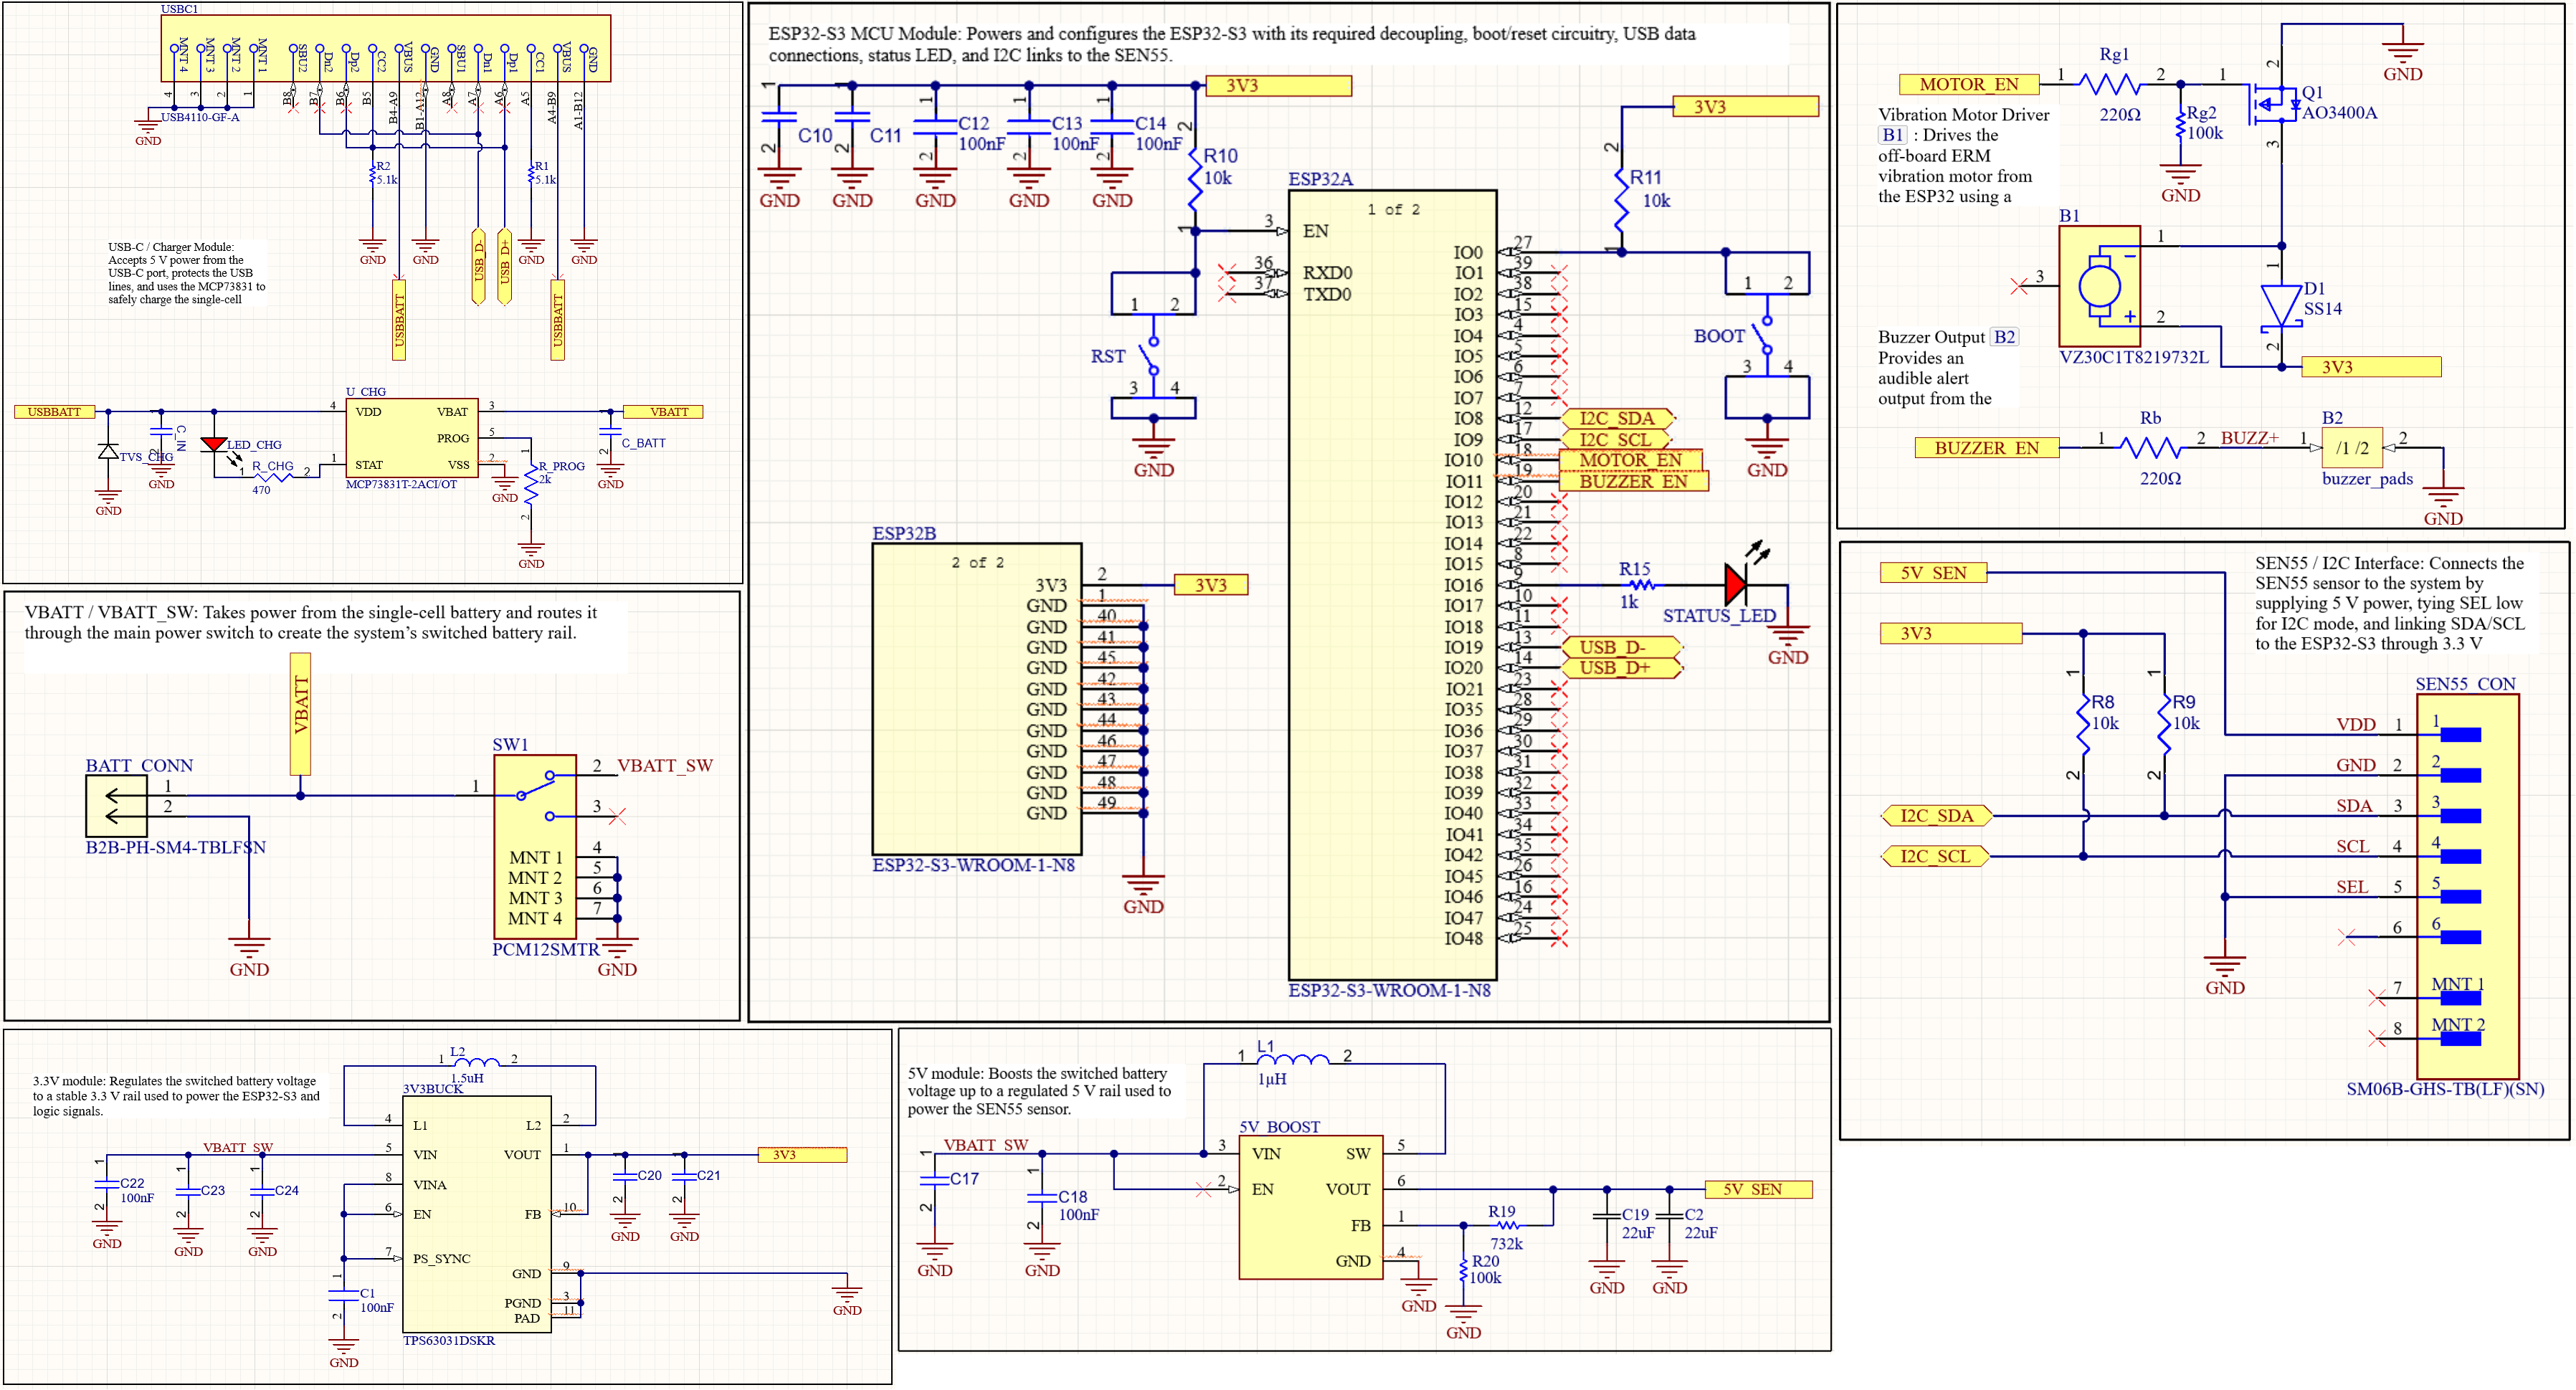
\includegraphics[width=\linewidth]{img/pcb_schematicfinal.drawio.png}
\vspace{0.4em}
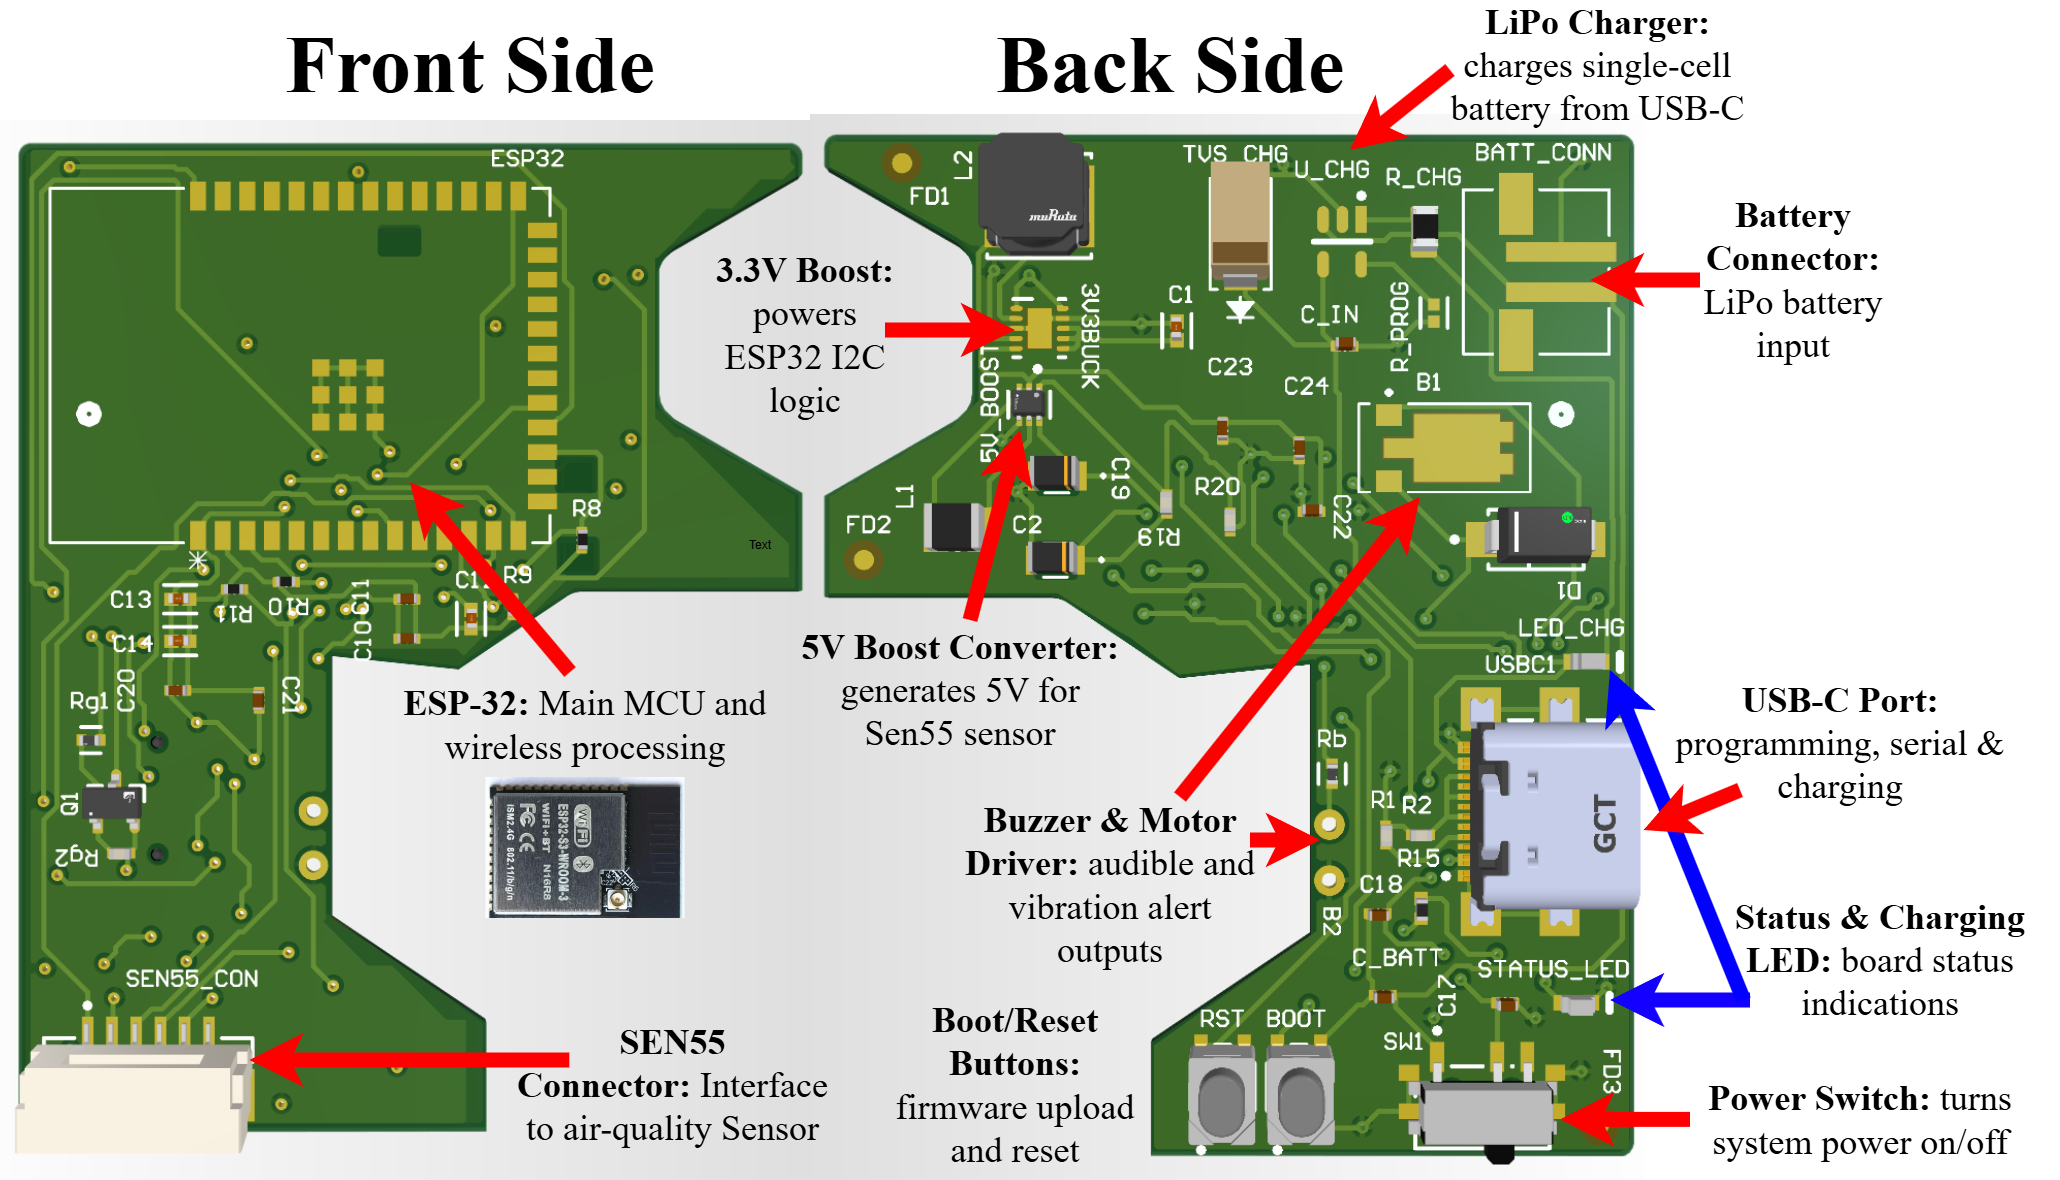
\includegraphics[width=\linewidth]{img/pcblabeled.drawio.png}
\end{card}

\end{column}

% =====================================================================
% MIDDLE COLUMN
% =====================================================================
\begin{column}{.315\linewidth}

\begin{card}{System Architecture}
\centering
\resizebox{\linewidth}{!}{%
\begin{tikzpicture}[
  font=\sffamily,
  node distance=0.7cm and 0.5cm,
  box/.style={
    rounded corners=10pt, draw=cpgreen, thick,
    fill=cpgreen, text=white, align=center,
    minimum width=5.2cm, minimum height=3.2cm, inner sep=6pt,
    font=\sffamily\bfseries\LARGE
  },
  ai/.style={box, fill=cpsage, draw=cpsage},
  alert/.style={box, fill=cpgold, draw=cpgold},
  ext/.style={box, fill=cpcharcoal, draw=cpcharcoal, minimum width=4.6cm},
  flow/.style={->, very thick, draw=cpgold},
]

% Row 1 inside container: SEN55 -> Clean -> Store
\node[box] (sen)   {SEN55 Sensor\\\normalfont\large PM1 / PM2.5 / PM4 / PM10\\ VOC, NO\textsubscript{x}\\ Temp, RH};
\node[box, right=of sen]   (clean) {Clean Up Data\\\normalfont\large Remove startup noise\\ Smooth readings\\ Adjust for T / RH};
\node[box, right=of clean] (store) {Store Recent Data\\\normalfont\large Rolling history of\\ recent readings};

% Row 2 inside container (snake R-to-L): Output <- AI <- Features
\node[box, below=1.6cm of sen]  (out)  {Output\\\normalfont\large Calibrated PM2.5\\ AQI category\\ GOOD $\rightarrow$ HAZARDOUS};
\node[ai,  below=1.6cm of clean] (ai)   {Tiny AI Model\\\normalfont\large Quantized CNN\\ on the ESP32-S3};
\node[box, below=1.6cm of store] (feat) {Feature Extraction\\\normalfont\large Trends and stats\\ from recent data};

% External boxes
\node[ext, left=of sen]   (pwr)    {Power System\\\normalfont\large USB-C charging\\ 5\,V / 3.3\,V rails};
\node[alert, below=2.2cm of out]  (alerts) {On-Device Alerts\\\normalfont\large Vibration motor\\ Piezo buzzer\\ Severity pulses};
\node[ext,   below=2.2cm of ai]   (dash)   {Dashboard \& BLE\\\normalfont\large BLE companion app\\ Serial monitor\\ Cloud sync};

% Container around inside nodes only — header sits above
\node[draw=cpgreen, ultra thick, rounded corners=16pt,
      fit=(sen)(clean)(store)(feat)(ai)(out),
      inner xsep=0.7cm, inner ysep=0.8cm] (esp) {};
\node[anchor=south, text=cpgreen, yshift=0.25cm,
      font=\sffamily\bfseries\Huge] at (esp.north) {ESP32-S3 On-Device Processing};

% Data flow (snake): sen -> clean -> store -> down -> feat -> ai -> out
\draw[flow] (sen)   -- (clean);
\draw[flow] (clean) -- (store);
\draw[flow] (store) -- (feat);
\draw[flow] (feat)  -- (ai);
\draw[flow] (ai)    -- (out);

% Output fans out to both consumers (outside container)
\draw[flow] (out)       -- (alerts);
\draw[flow] (out.south) |- (dash.west);

% Power feeds in from the left
\draw[flow] (pwr.east)  -- (sen.west);
\end{tikzpicture}%
}
\figcap{End-to-end data path. All calibration and classification run on
the ESP32-S3; the cloud is used only for visualization and long-term storage.}
\end{card}

\begin{card}{Embedded CNN Calibration}
A lightweight \textbf{1D convolutional network} runs continuously on the
ESP32-S3 to correct sensor drift and cross-sensitivity --- the core
research contribution of this project.
\vspace{0.3em}
\begin{itemize}\setlength\itemsep{0.25em}
  \item \textbf{Base model} trained on AQS reference-grade station data
  \item \textbf{Transfer learning} fine-tunes the head on local Sensa
        co-location data
  \item \textbf{Post-training int8 quantization} via TFLite Micro --- the model
        fits in ${<}\,100$\,KB of flash and runs in ${<}\,15$\,ms / inference
  \item Inference loop: \emph{SEN55 read $\rightarrow$ pre-process $\rightarrow$
        ring buffer $\rightarrow$ TFLite Micro $\rightarrow$ class + corrected PM}
\end{itemize}
\vspace{0.3em}
\centering
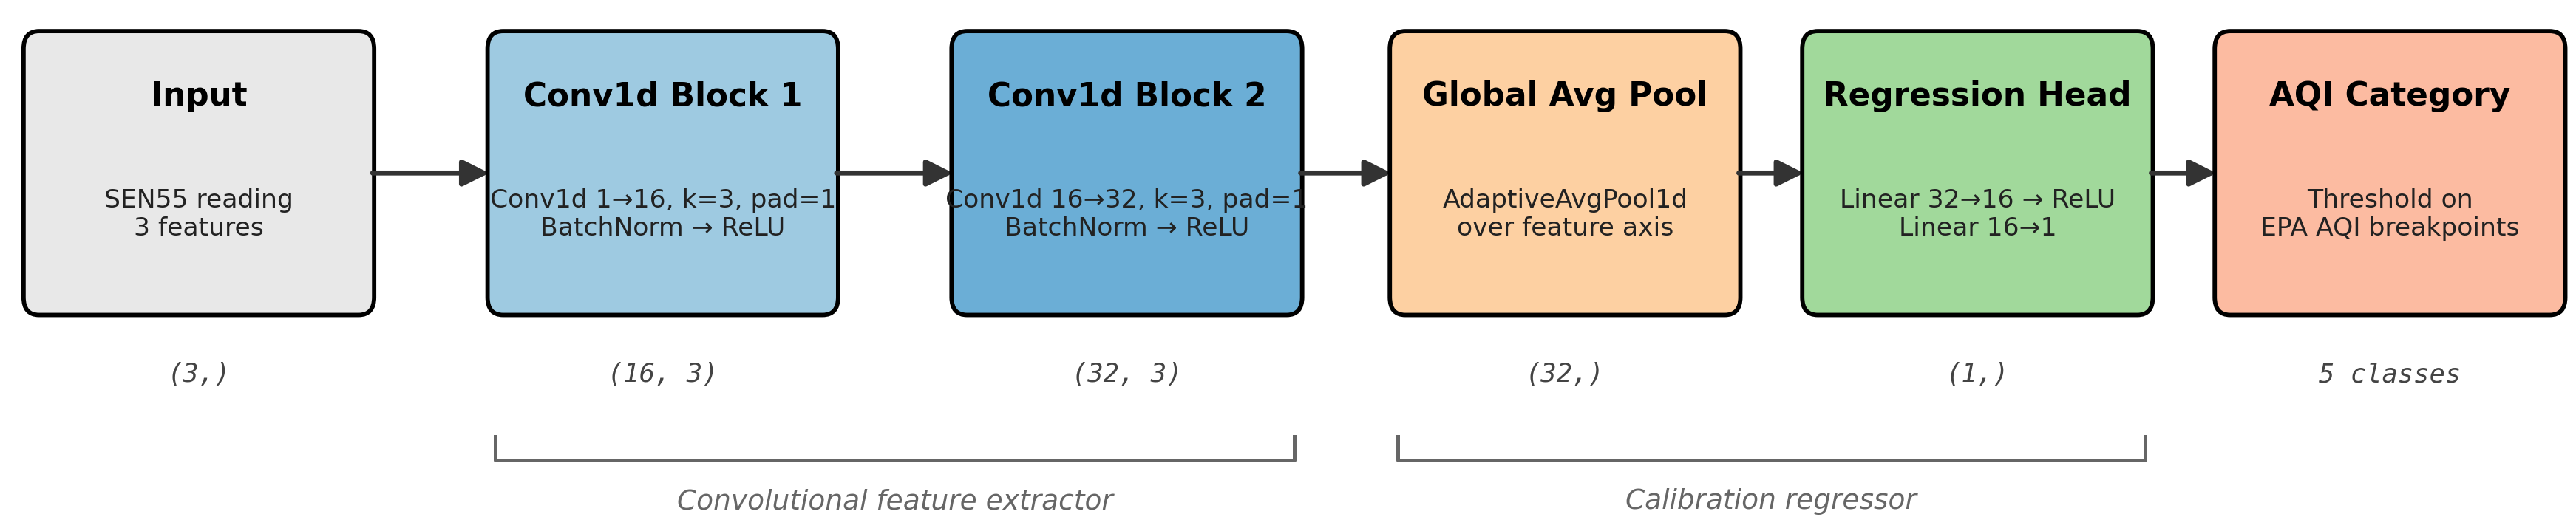
\includegraphics[width=\linewidth]{img/fig_cnn_architecture.png}
\figcap{CNN calibration uses transfer learning and physics informed AI to 
incorporate humidity and temperature into PM predictions Quantized 1D-CNN deployed on-device.}
\end{card}

\begin{card}{Severity-Coded Alerts}
When the on-device classifier flags poor air quality, the haptic motor and
piezo buzzer fire in a pattern that maps directly to AQI severity:
\vspace{0.3em}
\centering
\setlength{\tabcolsep}{1.0em}\renewcommand{\arraystretch}{1.25}
{\small
\begin{tabular}{lc}
\toprule
\textbf{Classification} & \textbf{Pulses} \\
\midrule
UNHEALTHY & 1 \\
VERY UNHEALTHY & 2 \\
HAZARDOUS & 3 \\
\bottomrule
\end{tabular}}
\justifying\vspace{0.4em}
A 30-second cooldown prevents alert fatigue when air quality remains poor.
\end{card}

\end{column}

% =====================================================================
% RIGHT COLUMN
% =====================================================================
\begin{column}{.315\linewidth}

\begin{card}{AI Analysis \& Insights}
\centering
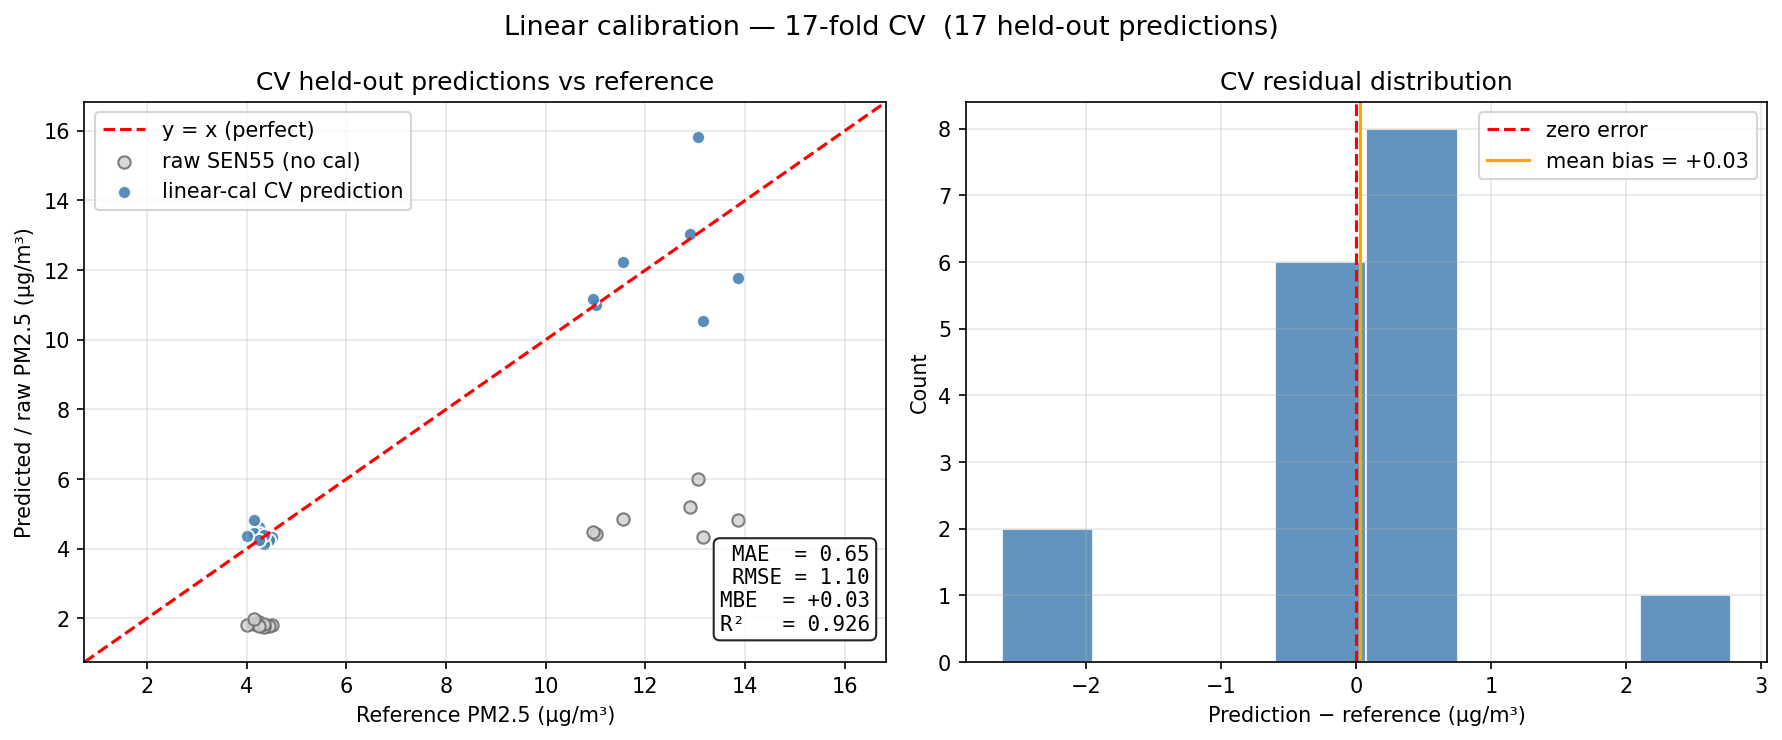
\includegraphics[width=\linewidth]{img/linear_cv_predictions_humidity.png}
\figcap{Reduced bias and error qualifies our sensor as "high-fidelity" under the stringent EPA guidelines that PurpleAir adheres to.}
\end{card}

\begin{card}{Web Dashboard}
\centering
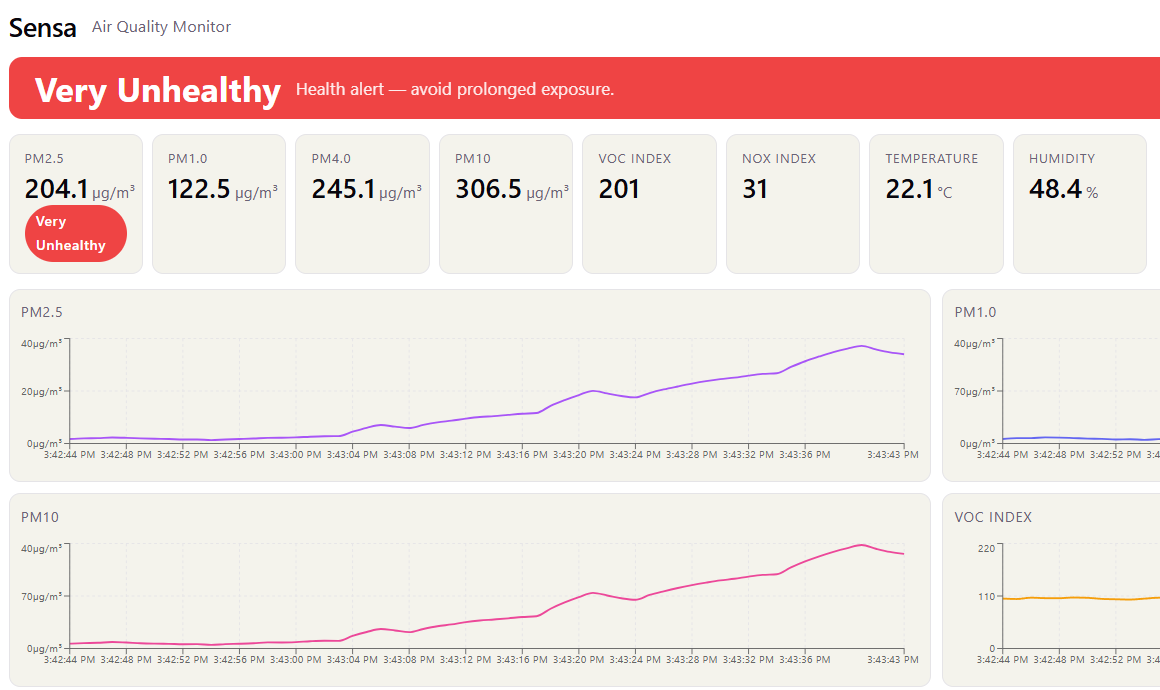
\includegraphics[width=\linewidth]{img/webappdemo.png}
\figcap{React / FastAPI dashboard renders the device's already-classified
output --- the AI runs on the wearable, not the server.}
\justifying\vspace{0.3em}
\begin{itemize}\setlength\itemsep{0.2em}
  \item Live readings stream over BLE $\rightarrow$ companion app $\rightarrow$ cloud
  \item Historical trends, exposure summaries, exportable CSV
  \item No raw PII --- only sensor data is uploaded
\end{itemize}
\end{card}

\begin{card}{Results \& Future Work}
\begin{itemize}\setlength\itemsep{0.3em}
  \item Embedded CNN calibration reduces PM\textsubscript{2.5} RMSE vs. raw SEN55
        output during co-location with reference equipment
  \item Full firmware fits in ${<}\,1$\,MB; CNN inference under 15\,ms
  \item Battery life meets the 12-hour target on a single LiPo cell
\end{itemize}
\vspace{0.3em}
\textbf{Next steps:}
\begin{itemize}\setlength\itemsep{0.2em}
  \item Extend transfer-learning pipeline to per-user adaptation
  \item Add NO\textsubscript{x} / VOC-specific calibration heads
  \item Long-duration field deployment (${>}\,30$ days)
\end{itemize}
\end{card}

\end{column}

\end{columns}
\end{frame}
\end{document}
